% last updated in April 2002 by Antje Endemann
% Based on CVPR 07 and LNCS, with modifications by DAF, AZ and elle, 2008 and AA, 2010, and CC, 2011; TT, 2014; AAS, 2016

\documentclass[runningheads]{llncs}
\usepackage{graphicx}
\usepackage{amsmath,amssymb} % define this before the line numbering.
\usepackage{ruler}
\usepackage{color}
\usepackage{epsfig}
\usepackage{graphics}
\usepackage{subfigure}


\usepackage[width=122mm,left=12mm,paperwidth=146mm,height=193mm,top=12mm,paperheight=217mm]{geometry}
\begin{document}
% \renewcommand\thelinenumber{\color[rgb]{0.2,0.5,0.8}\normalfont\sffamily\scriptsize\arabic{linenumber}\color[rgb]{0,0,0}}
% \renewcommand\makeLineNumber {\hss\thelinenumber\ \hspace{6mm} \rlap{\hskip\textwidth\ \hspace{6.5mm}\thelinenumber}}
% \linenumbers
\pagestyle{headings}
\mainmatter
\def\ECCV16SubNumber{496}  % Insert your submission number here

\title{Fully Convolutional Attention Localization Networks: Efficient Attention Localization for Fine-Grained Recognition} % Replace with your title

\titlerunning{ECCV-16 submission ID \ECCV16SubNumber}

\authorrunning{ECCV-16 submission ID \ECCV16SubNumber}

\author{Anonymous ECCV submission}
\institute{Paper ID \ECCV16SubNumber}


\maketitle

\begin{abstract}
Fine-grained recognition is challenging mainly because the inter-class differences between fine-grained classes are usually local and subtle while intra-class differences could be large due to pose variations.
In order to distinguish them from intra-class variations, it is essential to zoom in on highly discriminative local regions.
In this work, we introduce a reinforcement learning-based fully convolutional attention localization network to adaptively select multiple task-driven visual attention regions.
We show that zooming in on the selected attention regions significantly improves the performance of fine-grained recognition.
Compared to previous reinforcement learning-based models \cite{bd1,bd2,bd3}, the proposed approach is noticeably more computationally efficient during both training and testing
because of its fully-convolutional architecture, and it is capable of simultaneous focusing its glimpse on multiple visual attention regions.
The experiments demonstrate that the proposed method achieves notably higher classification accuracy on three benchmark fine-grained recognition datasets: Stanford Dogs \cite{bd4}, Stanford Cars \cite{bd5}, and CUB-200-2011 \cite{bd6}.
\keywords{Visual Attention, Fine-grained Recognition, Convolutional Neural Network, Reinforcement Learning}
\end{abstract}


%%%%%%%%% BODY TEXT
\section{Introduction}
Fine-grained recognition refers to the task of distinguishing sub-ordinate categories, such as bird species, dog breeds, and car models. It is an important topic to make computer rivals human experts in visual understanding.
Compared to generic object recognition, fine-grained recognition is more challenging,
because the discriminative features to recognize fine-grained classes are typically not just on the whole object but also on multiple object parts.
Therefore, it requires us to both locate the parts that contain discriminative details and differentiate fine details in appearance.

Most conventional methods~\cite{bd10,bd15} utilize manually defined parts to localize the regions, such as ``the head of a bird'', for fine-grained recognition.
Relying on manually defined parts has several drawbacks: 1) the precise part annotations is expensive to acquire.
2) The strongly supervised part-based model might fail if some parts are occluded.
3) Finally but most importantly, there is no clue that manually defined parts are optimal for all  fine-grained recognition tasks.
For example, it is very difficult to define parts for food recognition.


In this paper, we propose a novel framework called {\em Fully Convolutional Attention Localization Network} to locate object parts without any human annotation.
Our framework utilizes reinforcement learning-based visual attention model~\cite{bd1,bd3} to simultaneous learn to localize object parts and classify object within scene.
The framework simulate the recognition process of human system system by learning a task-driven policy to localize object parts via a set of {\em glimpse}.
Each glimpse corresponds to an object part.
It takes the original image as well as the locations of the previous glimpses as inputs, and outputs the next glimpse location as the next object part.
The framework requires no manual part annotations, and it can be learned in an end-to-end way by REINFORCE algorithm~\cite{bd20}, where the location of each glimpse is an action,
the image and the location of the previous glimpses are the state, and the reward measures the classification correctness.
The visual attention approach is demonstrated to perform well on fine-grained recognition without requiring manually labeled object parts~\cite{bd3}.

Compared to the previous reinforcement learning-based visual attention framework~\cite{bd1,bd3},
Fully Convolutional Attention Localization Network leads both better computational efficiency and higher classification accuracy in fine-grained recognition.
The previous framework is computationally expensive during both training and testing because it  needs to run a neural networks individually on each image crop.
In our framework, a glimpse is produced by passing the image to a fully convolutional neural network~\cite{bd7,bd8}.
The fully convolutional neural network generates a score map using the original image and the score maps of the last glimpses.
Each score map corresponds to an object part. Different parts can have different size.
The location with the maximum score is utilized as the attention region of the corresponding part.
The attention localization network enjoys very fast training and testing, because of its fully-convolutional architecture and feature sharing techniques.
The convolutional neural network is shared across multiple glimpses, and the convolutional neural networks of all the parts are also shared in a way similar to Fast-RCNN~\cite{girshick2015fast}.
The proposed framework is able to simultaneously locate multiple parts, while the previous frameworks~\cite{bd1,bd3} generally only locate one part.
As a result, the proposed approach outperforms state-of-the-art reinforcement~\cite{bd1,bd3} learning-based approaches in fine-grained recognition accuracy by a large margin.

We perform experimental evaluation on three publicly available datasets: Stanford Dogs \cite{bd4}, Stanford Cars \cite{bd5} and CUB-200-2011 \cite{bd6}.
The experiments demonstrate that the proposed framework can improve the performance significantly over state-of-the-art reinforcement learning based methods without utilizing external data or complicated model fusion techniques.
It also outperforms most previous state-of-the-art methods on Stanford Dogs ($84.1\%$ vs $82.6\%$).

The remainder of the paper is organized as follows. The related work is reviewed in Section 2.
The architecture of fully convolutional attention localization network is described in Section 3.
The training process of the proposed framework is described in Section 4.
The implementation details, performance studies, and experimental analysis are illustrated in Section 5.
The conclusion and future work is presented in Section 6.

\section{Related Work}
\subsection{Fine-Grained Recognition}
Fine-grained recognition algorithms rely on part localization~\cite{bd9,bd10,bd11,bd12,bd13,bd14} to focus on the important regions and discriminative representation learning to distinguish the subtle difference.

Part localization-based fine-grained recognition algorithms localize important regions using a set of predefined parts, which can either be manually defined or automatically found using data mining techniques.
Most of the algorithms employs manually defined object parts.
Berg et al. \cite{bd9} learn a set of intermediate features using data mining techniques.
Each feature discriminates two classes based on the appearance of a particular part.
Liu et al. \cite{bd10} employ the local appearance features of manually defined parts, such as face and eyes, and combine them with global features for dog breed classification.
The experimental results show that accurate part localization considerably increases classification performance.
Zhang et al. \cite{bd11} utilize part-based R-CNNs as whole-object and part detectors to detect the pose of the objects.  The CNN appearance representation is then pose-normalized for fine-grained recognition.

Some other works that find discriminative parts in an unsupervised way.
Yang et al. \cite{bd12} propose a template model to discover the common geometric patterns of object parts and the co-occurrence statistics of the patterns.
Features are extracted within the aligned co-occurred patterns for fine-grained recognition.
Similarly, Gavves et al. \cite{bd13} and Chai et al. \cite{bd14} segment images and align the image segments in an unsupervised fashion.
The aligned image segments are utilized for feature extraction separately.

Successful fine-grained recognition also calls for discriminative representation learning to learn appearance feature.
Most of the current state-of-the-art fine-grained recognition algorithms are based on deep CNN representation.
Branson et al. \cite{bd15} claim that integrating lower-level layer and higher-level layer features learns more discriminative representation for fine-grained recognition.
Lin et al. \cite{bd16} propose a bilinear architecture to model local pairwise feature interactions for fine-grained recognition, where convolutional features from two models are combined in a translation invariant manner.
Qian et al. \cite{bd17} propose a multi-stage metric learning framework to learn a distance metric that pulls data points of the same class close and pushes data points from different classes far apart.
Wang et al. \cite{bd18} combine saliency-aware object detection approach and object-centric sampling scheme to extract more robust and discriminative features for large-scale fine-grained car classification.

Although these works have achieved major progresses on fine-grained recognition and demonstrated the importance of part localization and discriminative representation learning, most of them treat these two tasks separately,
and most of them require part annotations.

\subsection{Attention Model}
Several works introduce attention-based models for task-driven object/part localization.
Mnih et al. \cite{bd1} present a recurrent neural network model for object detection by adaptively selecting a sequence of attention regions and extract appearance  representations in the these regions.
Since this model is non-differentiable, it  is trained with reinforcement learning technique to learn  task-specific policies.
Ba et al. \cite{bd2} extend Mnih et al.'s work and successfully achieve good results on a more challenging multi-digit recognition task.
Sermanet et al.~\cite{bd3} further extend \cite{bd2} and present experiments on fine-grained recognition datasets.
Jaderberg et al.~\cite{jaderberg2015spatial} proposes an differentiable attention mechanism that does not need reinforcement learning for training.

Compared to previous approaches, the recurrent attention models \cite{bd1,bd2,bd3} have remarkable contributions to fine-grained recognition problem,
because they can learn the part localization and discriminative representation in an end-to-end way, and they do not require manually labeled object parts.
However, they also suffer from several drawbacks in practice. First, they only result in small performance improvement.
\cite{bd3}  achieves 76.8\% mean accuracy percentage (with 3 glimpses) on Stanford Dogs dataset while the result of GoogLeNet \cite{bd7} baseline is 75.5\%.
Second, the computational burden is high.
Calculating the features at each glimpse in \cite{bd3} requires forwarding GoogLeNet three times, leading to very slow training and testing.

The proposed framework improves the attention models in several aspects:
\begin{itemize}\vspace{-8pt}
\item {\bf Computational Efficiency:} It is much more computationally efficient because of the fully convolutional neural network architecture and feature sharing technique.
\item {\bf Multiple Part Localization:} It is capable of localizing multiple parts with different sizes simultaneously.
\end{itemize}

As a result, the proposed framework not only achieves noticeable improvements over state-of-the-art methods on several benchmark datasets,
it is also more suitable to be applied to  larger datasets, which is common in industrial applications, because of its computational efficiency.

% \begin{itemize}
% \item \textbf{Small performance improvement.} \cite{bd3}  achieves 76.8\% mean accuracy percentage (with 3 glimpses) on Stanford Dogs dataset while the result of GoogLeNet \cite{bd7} baseline is 75.5\%. Considering the attention-based model is much more complicated, the improvement is slight.

% \item \textbf{High computational burden.} \cite{bd3} employs GoogLeNet for representation learning. However, calculating the features at each glimpse requires forwarding GoogLeNet three times, leading to very slow training and testing.

% %\item \textbf{Convergence difficulty.} Because the attention-based models\cite{bd1,bd2,bd3} are trained with reinforcement learning, the convergence of the model is slow and heavily depends on the exploration parameters.
% \end{itemize}

% In contrast to the above works, the training and testing of the proposed work is much faster, and the recognition accuracy significantly outperforms the baseline methods.

\section{Fully Convolutional Attention Localization Networks}

\begin{figure*}[!t]
\begin{center}
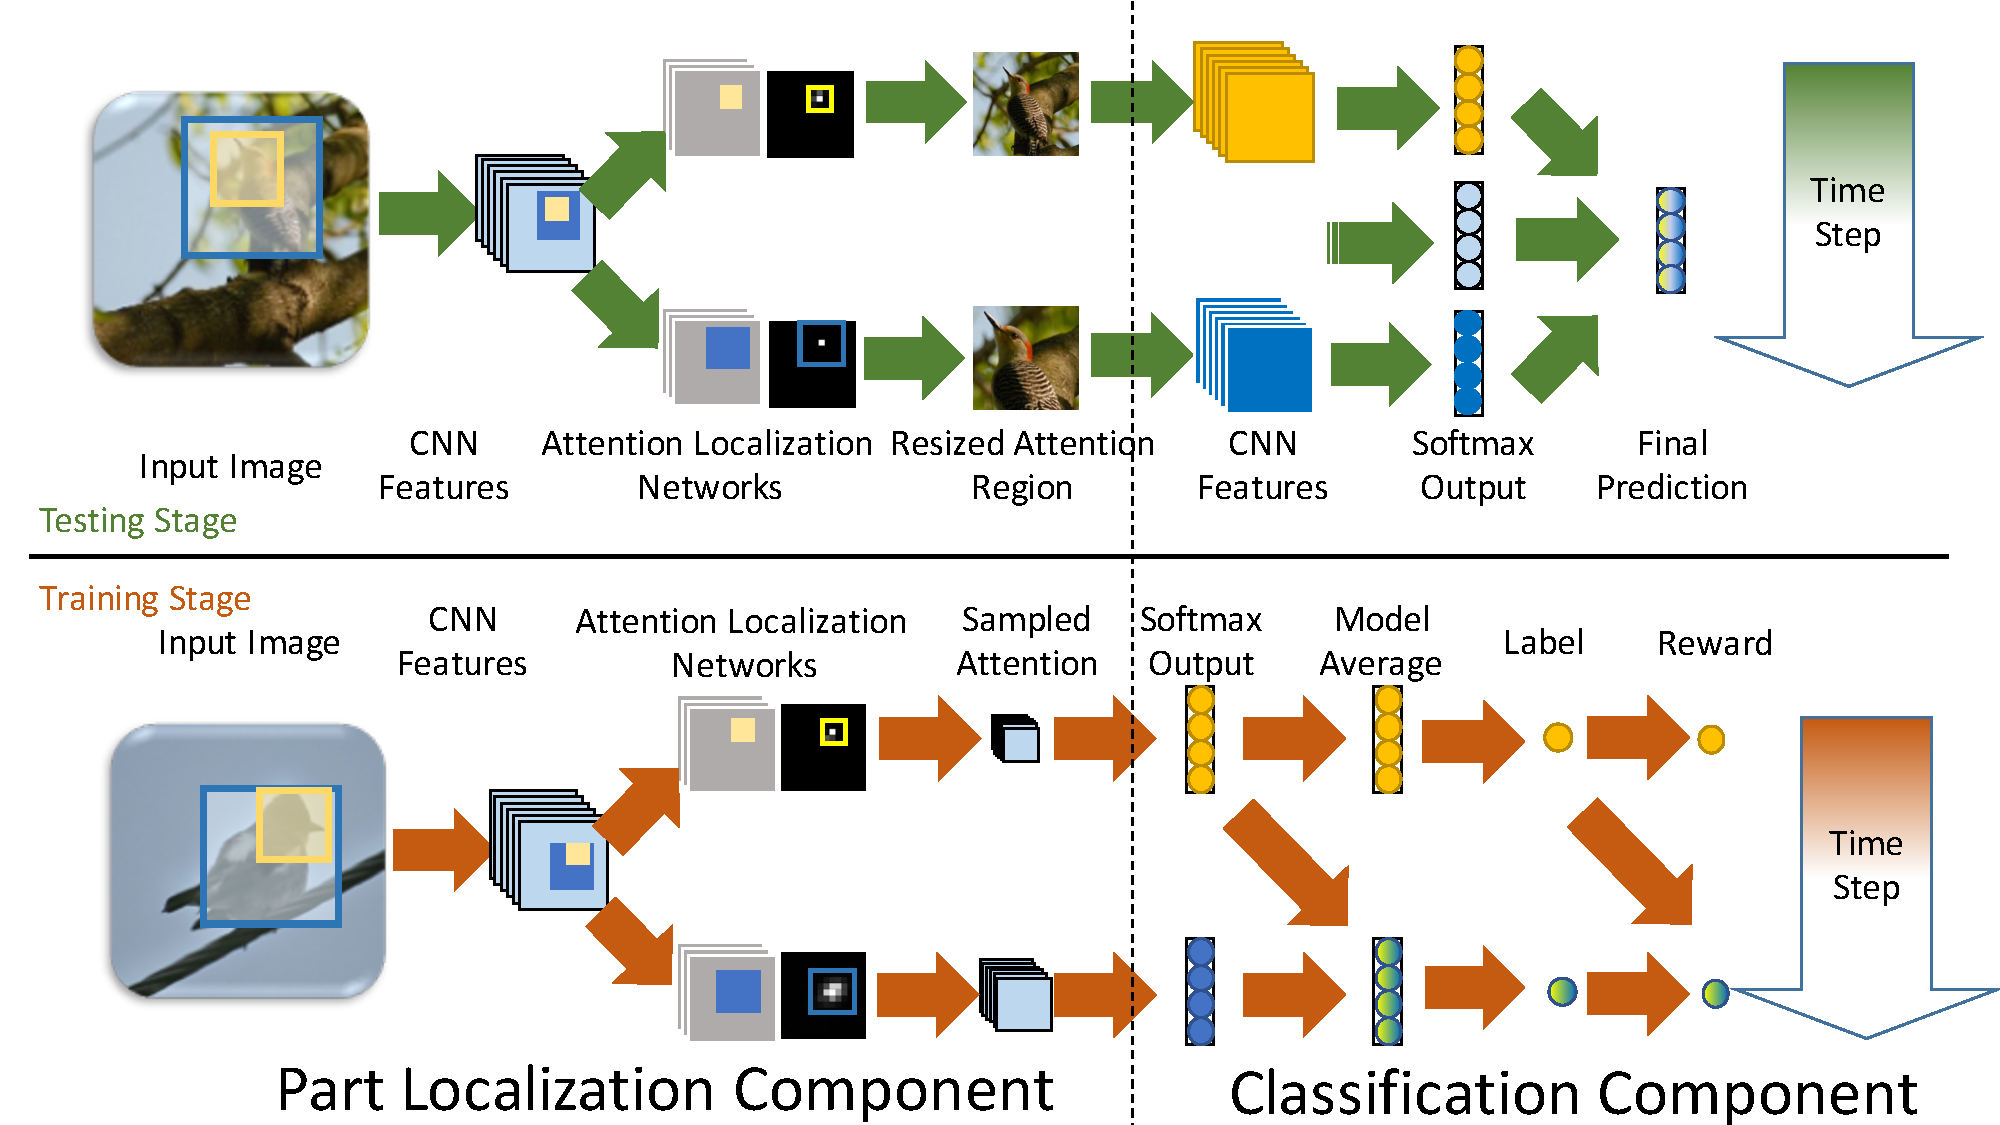
\includegraphics[width=4.8in]{1.pdf}
\end{center}
\caption{The architecture of the attention localization network. In this example, the attention localization network finds two parts with different sizes (the blue region and the yellow region).
The upper part shows the architecture for testing, and the lower part shows the architecture for training. In testing, each part is resized to high resolution for classification.
In training, the corresponding convolutional features in attention localization network is re-used for classification.
}\label{fig:architecture}
\vspace{-8pt}
\end{figure*}

Fig.~\ref{fig:architecture} illustrates the architecture of the Fully Convolutional Attention Localization Network.
The Fully Convolutional Attention Localization Network can localize multiple object parts using attention mechanism.
Different parts can have different pre-defined sizes.
The network contains two components: part localization component and classification component.

The part-localization component uses a fully-convolutional neural network to locate part locations.
Given an input image, we extract the basis convolutional feature maps using the VGG 16 model \cite{bd8} pretrained on ImageNet dataset~\cite{bd19} and fine-tuned for the target fine-grained dataset.
The attention localization network localizes multiple parts by generating a score map for each part using  the basis convolutional feature map.
Each score map is generated using two stacked convolutional layers and one spatial softmax layers.
The first convolutional layer uses 64 $3\times3$ kernels, and the second one uses one $3\times3$ kernels to output a single-channel confidence map.
The spatial softmax layer is applied to the confidence map to convert the confidence score into probability.
The attention region with highest probability is selected as the part location.
The same process are applied for a fixed number of timesteps for multiple part locations.
Each timestep generates the location for a particular part.

The classification component contains one deep CNN classifier for each part as well as the whole image.
Different part might have different size, and a local image region is cropped around each part location according to its size.
We train an image classifier for each local image region as well as the whole image separately.
The final classification results is the average of all the classification results from the individual classifiers.
In order to discriminate the subtle visual differences, each local image region is resized to high resolution.
A  deep convolutional neural network is trained for each part for classification separately.


Although resizing local image regions can achieve good classification performance, it requires us to perform multiple forward and backward passes of $N$ very deep convolutional neural network in one batch during training, where $N$ is the number of parts. This is too time-consuming in practice.
Thus, we employ an approximated part classification method that is similar to Fast-RCNN~\cite{girshick2015fast} during training.
The convolutional feature maps for part localization, part classification, and whole image classification are shared during training.
The convolutional features for each part is obtained by selecting the corresponding region in the convolutional feature map of the whole image, so that the receptive field of the selected region is the same as the size of the part.
The convolutional features for all time steps are also shared.
As a result, we only need to run the forward pass of the deep convolutional once in one training batch.
Notice that these classification networks are only utilized to obtain the reward during attention localization network training.
The final classification networks are based on the resized high resolution images.

\subsection{Inference}
We now describe how to utilize the attention localization network for fine-grained recognition during inference.
As shown in Fig.~\ref{fig:architecture}, given an image, we first localize multiple attention regions by selecting the location with highest probability for each part in attention localization network.

We then zoom in on each part's location by resizing the regions around it to its corresponding high resolution.
Each resized part region as well as the original image makes the prediction individually using the classification part.
The final prediction score is the average of the prediction scores from the original image and all the attention regions.


\section{Training Attention Localization Networks}
Since there are no ground-truth annotations to indicate where to select attention regions, we adopt reinforcement learning to learn the attention localization networks.

The entire attention localization problem is formulated into Markov Decision Processes (MDPs).
During each step of MDP, an attention localization network works as an agent to perform an action based on the observation and receives a reward.
In our work, the action corresponds to the location of the attention region, the observation is the input image and the crops of the attention regions,
and the reward measures the quality of the classification using the attention region.
The target of our learning is to learn the optimal decision policy to generate actions from observations,
characterized by the parameters of the attention localization networks, to maximize the sum of expected reward of all the timesteps.

In our work, additional auxiliary classification networks are trained to measure the classification quality.
The classification network in each step is a fully convolutional layer followed by a softmax layer,
which uses the attention maps of all the parts in the last timestep as well as the convolutional features of the whole image as the input.


The classification networks and the attention localization networks are jointly optimized to maximize the following objective function:
\begin{equation}
J(\theta_L, \theta_C) =  R(\theta_L) - \lambda L(\theta_C),
\end{equation}
where $\theta_L, \theta_C$ are the parameters of attention localization networks and classification networks, respectively.
Notice that we employ an approximated part classification method that is similar to Fast-RCNN~\cite{girshick2015fast} during training.
$\lambda$ is a balance weight,  $L(\theta_C)$ is the cross-entropy classification loss, and
\begin{equation}
R(\theta_L) = \frac{1}{NT}\sum_{n=1}^{N}\sum_{t=1}^T E_{\theta_L}(r_{n,t})
\end{equation}
is the average expected reward over $N$ training samples and $T$ different selection regions.

\begin{equation}
E_{\theta_L}(r_{n,t}) = \int_{A_{n,t}} p_{\theta_{L,t}}(A_{n,t}|x_n)r(A_{n,t})
\end{equation}
is the expected reward of the t-th selected attention region of the n-th sample,
where $\theta_{L,t}$ is the parameters of the t-th attention localization network,
$x_n$ is the n-th input image, and $A_{n,t}$ is the t-th selected region.
$p_{\theta_{L,t}}(A_{n,t}|x_n)$ is the probability of selecting $A_{n,t}$ as attention region.
The reward function $r(A_{n,t})$ is crucial for developing an efficient learning algorithm. We will describe the design of the reward function in the following subsection.

\subsection{Reward Strategy}
A straightforward reward strategy is to measure the quality of attention region selection policy as a whole using the final classification result,
i.e., $r(A_{n,t}) = 1$  if $t = T$ and the image is correctly classified, and 0 otherwise.
Although the MDP with such a reward strategy can be learned in a recurrent way \cite{bd1}, it confuses the effects of the selected regions in different timesteps,
and it might lead to the problem of convergence difficulty.

We consider an alternative reward strategy, namely greedy reward:
\begin{equation}
r(A_{n,t})=\left\{\begin{array}{ccc} 1 & : & t = 1 \wedge c_{n,1} = y_{n} \\ 1 &:& t > 1 \wedge c_{n,t} = y_{n} \wedge l_{n,t} < l_{n,t-1} \\ 0&:& otherwise   \end{array}\right.
\end{equation}
where $c_{n,t}$ is the predicted classification result, $y_{n}$ is the ground-truth label, and $l_{n,t}$ is the classification loss. If the image is classified correctly in the first step, the attention localization network immediately receives a reward. In other steps, we reward the corresponding attention localization network only if the image is classified correctly and the classification loss decreases with regards to the last timestep.
Otherwise, the attention localization network receives zero reward.

Since we immediately receive a reward when an image can be correctly classified using the current attention regions, the convergence of training is much easier and faster.

\subsection{Optimization}

\begin{figure}[htb]
  \begin{center}
    \subfigure[Forwarding]{
    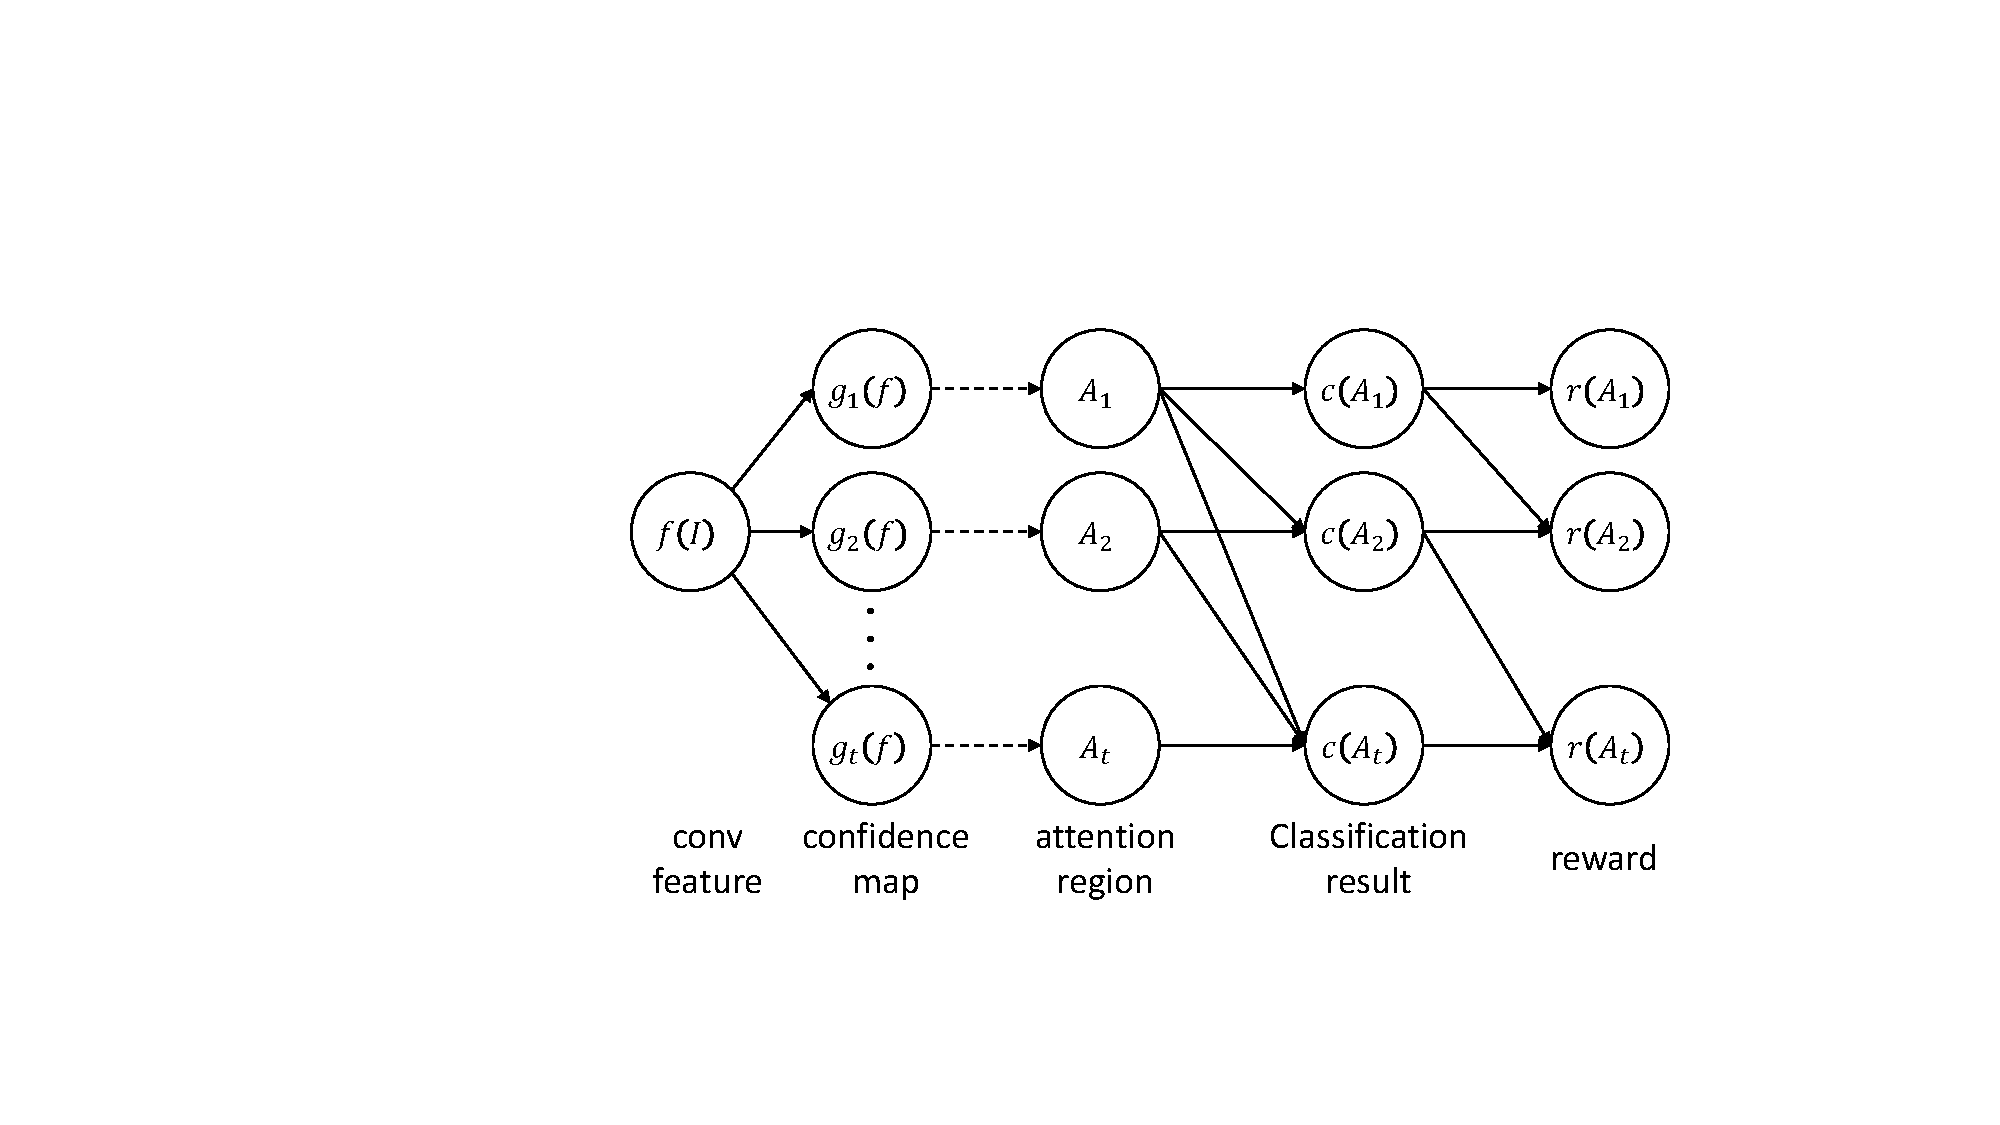
\includegraphics[scale = 0.3]{2-1.pdf}}
    \hspace{0.05in}%
    \subfigure[Back-propagation]{
    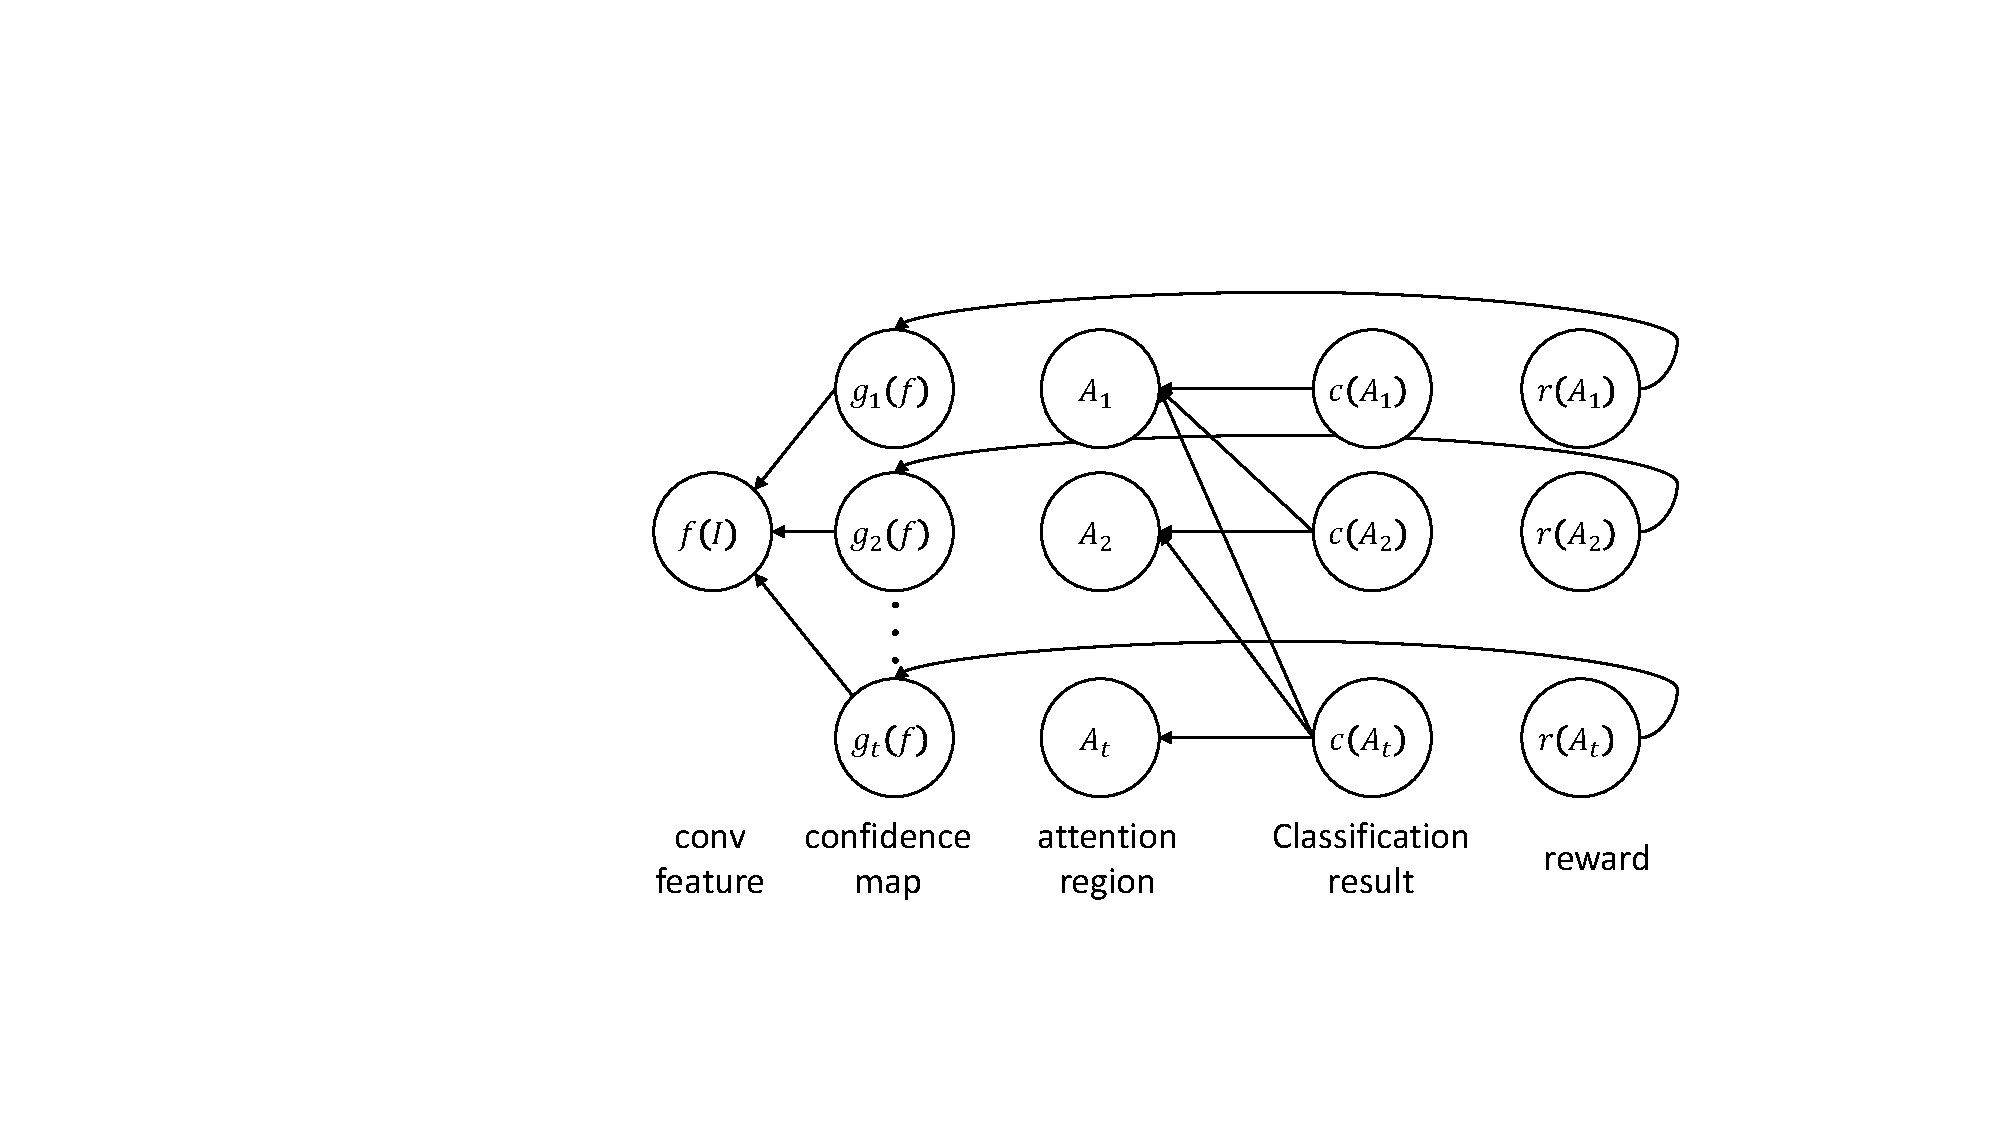
\includegraphics[scale = 0.3]{2-2.pdf}}
  \end{center}
\caption{The forwarding (a) and back-propagation (b) processes for training attention localization networks as MDPs. The dashed lines indicate the sampling procedures. }
\end{figure}

It is difficult to directly calculate the gradient of $E_{\theta_L}(r_{n,t})$ over $\theta_L$ because it requires evaluating exponentially many possible part locations during training.
As shown by \cite{bd20}, the gradient can be approximated in a Monte Carlo way:
\begin{eqnarray}
\partial (p_{\theta_{L,t}}(A_{n,t}|x_n)r(A_{n,t})) \hspace{1.3in}\\
= p_{\theta_{L,t}}(A_{n,t}|x_n) \partial (\log p_{\theta_{L,t}}(A_{n,t}|x_n)r(A_{n,t})) , \nonumber
\end{eqnarray}
Thus,
\begin{eqnarray}
\partial E_{\theta_L}(r_{n,t}) \hspace{2.1in}\\
 = \int_{A_{n,t}} p_{\theta_{L,t}}(A_{n,t}|x_n) \partial (\log p_{\theta_{L,t}}(A_{n,t}|x_n)r(A_{n,t})) \hspace{-0.215in} \nonumber\\
 \approx \frac{1}{K} \sum_{k=1}^K \partial(\log p_{\theta_{L,t}}(A_{n,t}^k|x_n)r(A_{n,t}^k)) \hspace{0.5in} \nonumber
\end{eqnarray}
where $A_{n,t}^k\sim p_{\theta_{L,t}}(A_{n,t}|x_n) $ is sampled according to a multinomial distribution parameterized by the output confidence map of the attention localization network.

The forwarding process of training the attention localization networks as MDPs is shown in Figure 2(a). Given basis conv features $f(I)$ as input, the attention networks output the confidence map $g_t(f)$ for different time step. Each confidence map $g_t(f)$ forms a multinomial distribution, and the location of attention region $A_t$ is sampled under the distribution. The sampling procedure is repeated for $K$ times. We can then use them for classification $c(A_t)$, and further get the reward $r(A_t)$.

During back-propagation, the gradient $\partial L(\theta_C)$ can be  obtained by the back-propagation in the classification networks.
The gradient $\partial R(\theta_L)$ is calculated using policy gradient (6).
Notice that when the reward is 0, we can just ignore the sample.

\section{Experiments}
We conduct extensive experiments on the Stanford Dogs \cite{bd4}, Stanford Cars \cite{bd5} and CUB-200-2011 \cite{bd6} datasets.
Table 1 shows the statistics of the three datasets.

\begin{table*}[htb]
\begin{center}
\begin{tabular}
{c|c|c|c|c|c}\hline
Dataset & class & train & test & bounding box & part annotation   \\\hline\hline
Stanford Dogs & 120 & 12,000  &  8,580 & $\surd$ &    \\
Stanford Cars & 196 & 8,144  & 8,041 & $\surd$ &  \\
CUB-200-2011 & 200 & 5,994 & 5,794 & $\surd$ & $\surd$ \\\hline
\end{tabular}
\caption{Statistics of the three datasets.}
\vspace{-20pt}
\end{center}
\end{table*}

\subsection{Implementation Details}
Although jointly training the entire model is possible, we develop a 3-step algorithm for the sake of training speed.
In the first step, we initialize and fine-tune the CNN model for extracting the basis convolutional feature maps for attention localization.
In the second step, we fix and cache the basis convolutional feature maps from the first step, and train the attention localization networks separately.
In the third step, we fix and cache the selected attention regions from the second step, and fine-tune the final classification models.
Through feature caching, repeated feature calculating is avoided.
Notice that the convolutional neural networks for attention localization and the final classification is different, though they are initialized similarly during pre-training described below.
We repeat these steps several times until convergence.

We use RMSProp to optimize the attention localization network with minibatches size 512, initial learning rate 0.01 and sampling number per step 16.

For the Stanford Dogs dataset, the VGG-16 \cite{bd8} network architecture is utilized to the CNN of both attention localization CNN and final classification.
During pre-training, we first scale all images to $256 \times256 $ resolution, and fine-tune the VGG-16 net (with randomly cropped $224\times224$ patches).
For each input image, the VGG-16 net outputs a $512\times16\times16$ conv5\_3 feature map.
We then use the feature map to train the attention localization network to find two parts.
The first part selects a $4\times4$ region in the feature map (correspond to a $64\times64$ patch in the original image), and the second one selects a $8\times8$ region in the feature map (correspond to a $128\times128$ patch in the original image).
The two resulted attention patches are resized to $256\times256$ to train VGG-16 prediction models in the final classification stage.

We use a different experimental  setting for the Stanford Cars and CUB-200-2011 dataset because most previous methods on them take higher resolution inputs.
Specifically, the input images are resized to $512\times512$ pixels.
To enable larger training batch, GoogLeNet \cite{bd7}  is used to extract the convolutional features.
For each $512\times512$ input image, the GoogLeNet outputs a $512\times16\times16$ inception\_5b/output conv feature map.
We then train attention localization networks to select $4\times4$ and $8\times8$ attention regions in the feature maps.
During final classification, the attention regions and the original images are resized to $448\times448$ for prediction.
We use $12\times12$ instead of $7\times7$ average pooling for the GoogLeNet to fit higher resolution inputs.

\subsection{Stanford Dogs}
We evaluate our approach on the Stanford Dogs dataset with different model variations.
The results are summarized in Table 2.
The fine-tuned baseline VGG-16 model takes the original image as input and achieves $76.7\%$ recognition accuracy.
Using $8\times8$ attention regions improves the accuracy to $81.4\%$.
If we combine the prediction results of original image and the $8\times8$ attention region, the result is improved to $84.0\%$.
Combining both attention regions and the original image further improves the result to $84.2\%$.
Bounding box annotations are not used for this dataset, and samples of selected attention regions are listed in Figure 3.

The proposed attention localization network takes 3 hours to converge on a K40 GPU, while the recurrent attention model \cite{bd3} takes about 30 hours for converging on the same dataset in our implementation (fine-tuning the conv features requiring additional training time for both models). Our testing time is 150ms, and the cost of attention selection is negligible compared with the feature calculation time, while recurrent attention model \cite{bd3} takes 250ms for testing in our implementation.

Since our approach is three times more expensive than a single VGG-16 model during testing, two additional model-fusion experiments are conducted to demonstrate its superiority.
In the multi-view test experiment, we evaluate the baseline VGG-16 model with three views.
For each input image, the prediction results of the full image and two random crops are combined to make the final prediction.
In the rigid combination experiment, we select the center  two regions of an image as well as the full image as attention regions, and the other processes are the same of the proposed approach.
The sizes of the crops is the same as the sizes of the parts in the attention model.
As shown in Table 2, when costing the same amount of testing time, using the attention regions outperforms multi-view test and rigid combination by a large margin.



\begin{table}[htb]
\begin{center}
\begin{tabular}
{c|c}\hline
Method &   Acc(\%) \\\hline\hline
VGG-16 original  & 76.7 \\
$8\times8$ Attention  & 81.4 \\
Original + $8\times8$ Attention & 84.0 \\
Original + $4\times4$, $8\times8$ Attention & 84.2 \\
Multi-view test  & 78.1 \\
Rigid combination & 77.1 \\\hline
\end{tabular}
\caption{Recognition results on the Stanford Dogs dataset with different settings.}
\vspace{-20pt}
\end{center}
\end{table}

We also compare the proposed framework with previous state-of-the-art methods in Table 3.
Gavves et al. \cite{bd13} utilize ground-truth bounding boxes during training and testing, but the results is only $50.1\%$.
Karuse et al. \cite{bd21} achieves a competitive $82.6\%$ accuracy, as the expense of using additional web-data from Google Image Search.
Sermanet et al. \cite{bd3} utilize reinforcement learning-based recurrent attention models, which is similar to our approach, but its recognition accuracy is $76.8\%$.

Figure 3 provides a qualitative comparison between the selected attention regions of the proposed framework and the recurrent attention models \cite{bd3}.
In both methods, we scale the input images to the same resolution for a fair comparison, and we illustrate two attention regions.
We can observe that both methods focus on reasonable attention regions, but our approach can select attention regions corresponding different semantic ``parts'' because of its well-designed reward strategy and network architecture.


\begin{table}[htb]
\begin{center}
\begin{tabular}
{c||c|c|c}\hline
Method &  bbox & web data & Acc(\%) \\\hline\hline
Ours &  & & 84.2 \\\
J. Krause et al. \cite{bd21} &  & $\surd$ & 82.6 \\
Gavves et al. \cite{bd13} & $\surd$ &  & 50.1 \\
Sermanet et al. \cite{bd3}  &  & & 76.8  \\\hline
\end{tabular}
\caption{Experimental results on the Stanford Dogs dataset.}
\vspace{-8pt}
\end{center}
\end{table}

\subsection{Stanford Cars}
The experimental results on the Stanford Cars dataset with different settings are summarized in Table 4.
The baseline GoogLeNet model takes the original image (resized to $448\times448$) as input and achieves $84.9\%$ recognition accuracy.
The attention model with an $8\times8$ attention regions as input obtain recognition accuracy of $80.1\%$.
Combining the prediction results of both the original image and an $8\times8$ attention region improves the result to $88.3\%$.
Combining two attention regions and the original image further improves the result to $89.1\%$.
Using the ground-truth bounding boxes as the attention regions further improves the result to $91.3\%$.
Some examples of selected attention regions are illustrated in Figure 3.

\begin{table}[htb]
\begin{center}
\begin{tabular}
{c|c}\hline
Method &   Acc(\%) \\\hline\hline
GoogLeNet  & 84.9 \\
$8\times8$ Attention  & 80.1 \\
Original + $8\times8$ Attention & 88.3 \\
Original + $4\times4$, $8\times8$ attention & 89.1 \\
Multi-view test  & 85.9 \\
Rigid combination & 86.3 \\\hline
\end{tabular}
\caption{Recognition results on the Stanford Cars dataset with different settings.}
\vspace{-8pt}
\end{center}
\end{table}

We also compare the proposed method with the previous state-of-the-art methods in Table 5.
Karuse et al. \cite{bd21} achieves $92.8\%$ accuracy and Lin et al. \cite{bd16} achieves $91.3\%$ without using bounding boxes.
Although the result of the proposed is not the best one on this dataset, it is simpler to implement than \cite{bd21} and uses less time for training and testing than \cite{bd16}.

\begin{table}[htb]
\begin{center}
\begin{tabular}
{c||c|c}\hline
Method &  bbox & Acc(\%) \\\hline\hline
Ours(without BB) &  & 89.1 \\\
Ours(with BB) & $\surd$ & 91.3 \\\
J. Krause et al. \cite{bd22} &  $\surd$ & 92.8 \\
Lin et al. \cite{bd16} &  & 91.3 \\
Girshick et al. \cite{bd24} & $\surd$ & 88.4 \\
Chai et al. \cite{bd25} & $\surd$  & 78.0 \\\hline
\end{tabular}
\caption{Experimental results on the Stanford Cars dataset.}
\vspace{-12pt}
\end{center}
\end{table}

\subsection{CUB-200-2011}
The results on CUB-200-2011 dataset with different settings are summarized in Table 6.
The recognition accuracy  of the baseline model is $77.6\%$.
Combining  the baseline model with the model that uses an $8\times8$ attention region improves the result to $81.6\%$, and adding two attention regions improves the result to $82.0\%$.
Using ground-truth bounding boxes as attention regions leads to the recognition accuracy of $84.3\%$.
Comparisons with other state-of-the-art methods are summarized in Table 7. Xu et al. \cite{bd23} use additional web data for training and achieve slight higher performance ($0.3\%$) than the proposed method. Lin et al. \cite{bd16} obtains the highest recognition accuracy ($85.1\%$) at the cost of constructing high dimension bilinear feature vectors, which makes the training procedure extremely slow and limits its application for larger dataset.

\begin{table}[htb]
\begin{center}
\begin{tabular}
{c|c}\hline
Method &   Acc(\%) \\\hline\hline
GoogLeNet  & 77.6 \\
$8\times8$ Attention  & 76.1 \\
Original + $8\times8$ Attention & 81.6 \\
Original + $4\times4$, $8\times8$ attention & 82.0 \\
Multi-view test  & 78.9 \\
Rigid combination & 79.0 \\\hline
\end{tabular}
\caption{Recognition results on the CUB-200-2011 dataset with different settings.}
\vspace{-20pt}
\end{center}
\end{table}

\begin{table}[htb]
\begin{center}
\begin{tabular}
{c||c|c|c|c}\hline
Method &  bbox & parts & web data & Acc(\%) \\\hline\hline
Ours(without BB) &  &   &   &82.0 \\\
Ours(with BB) & $\surd$ & &   & 84.3 \\\
J. Krause et al. \cite{bd22} &  $\surd$ &  &  & 82.8 \\
Lin et al. \cite{bd16} & $\surd$ &    &   & 85.1 \\
Xu et al. \cite{bd23} & $\surd$ & $\surd$ & $\surd$ & 84.6 \\
Zhang et al. \cite{bd11} & $\surd$ & $\surd$ &   & 73.9 \\
L. Liu et al. \cite{bd26}     & $\surd$ &   &   & 73.5 \\                \hline
\end{tabular}
\caption{Experimental results on the CUB-200-2011 dataset.}
\vspace{-12pt}
\end{center}
\end{table}

\subsection{Attention Visualization}
Fig.~\ref{fig:attention_illustration} shows the visualization of the attention regions generated by the proposed model and \cite{bd3}.
Both models can produce attention that focus on discriminative image regions.
It can be observed that different object parts correspond to different image regions in the proposed model, while the attention regions of the multiple steps in \cite{bd3} generally focus on only one region.
The attention map of the generated model is also more diverse than the attention map in \cite{bd3}.

Fig.~\ref{fig:attention_illustration2} further illustrates the part selection ability of attention localization network for fine-grained recognition.
In Fig.~\ref{fig:attention_illustration2}(a), the baseline GoogLeNet misclassifies the bird in the top row as a Rhinoceros Auklet which is the category of the bird in the bottom row. In Fig.~\ref{fig:attention_illustration2}(b), the attention localization network selects the beak and eye area as attention regions, and successfully distinguishes the two birds.

\begin{figure*}[!t]
\begin{center}
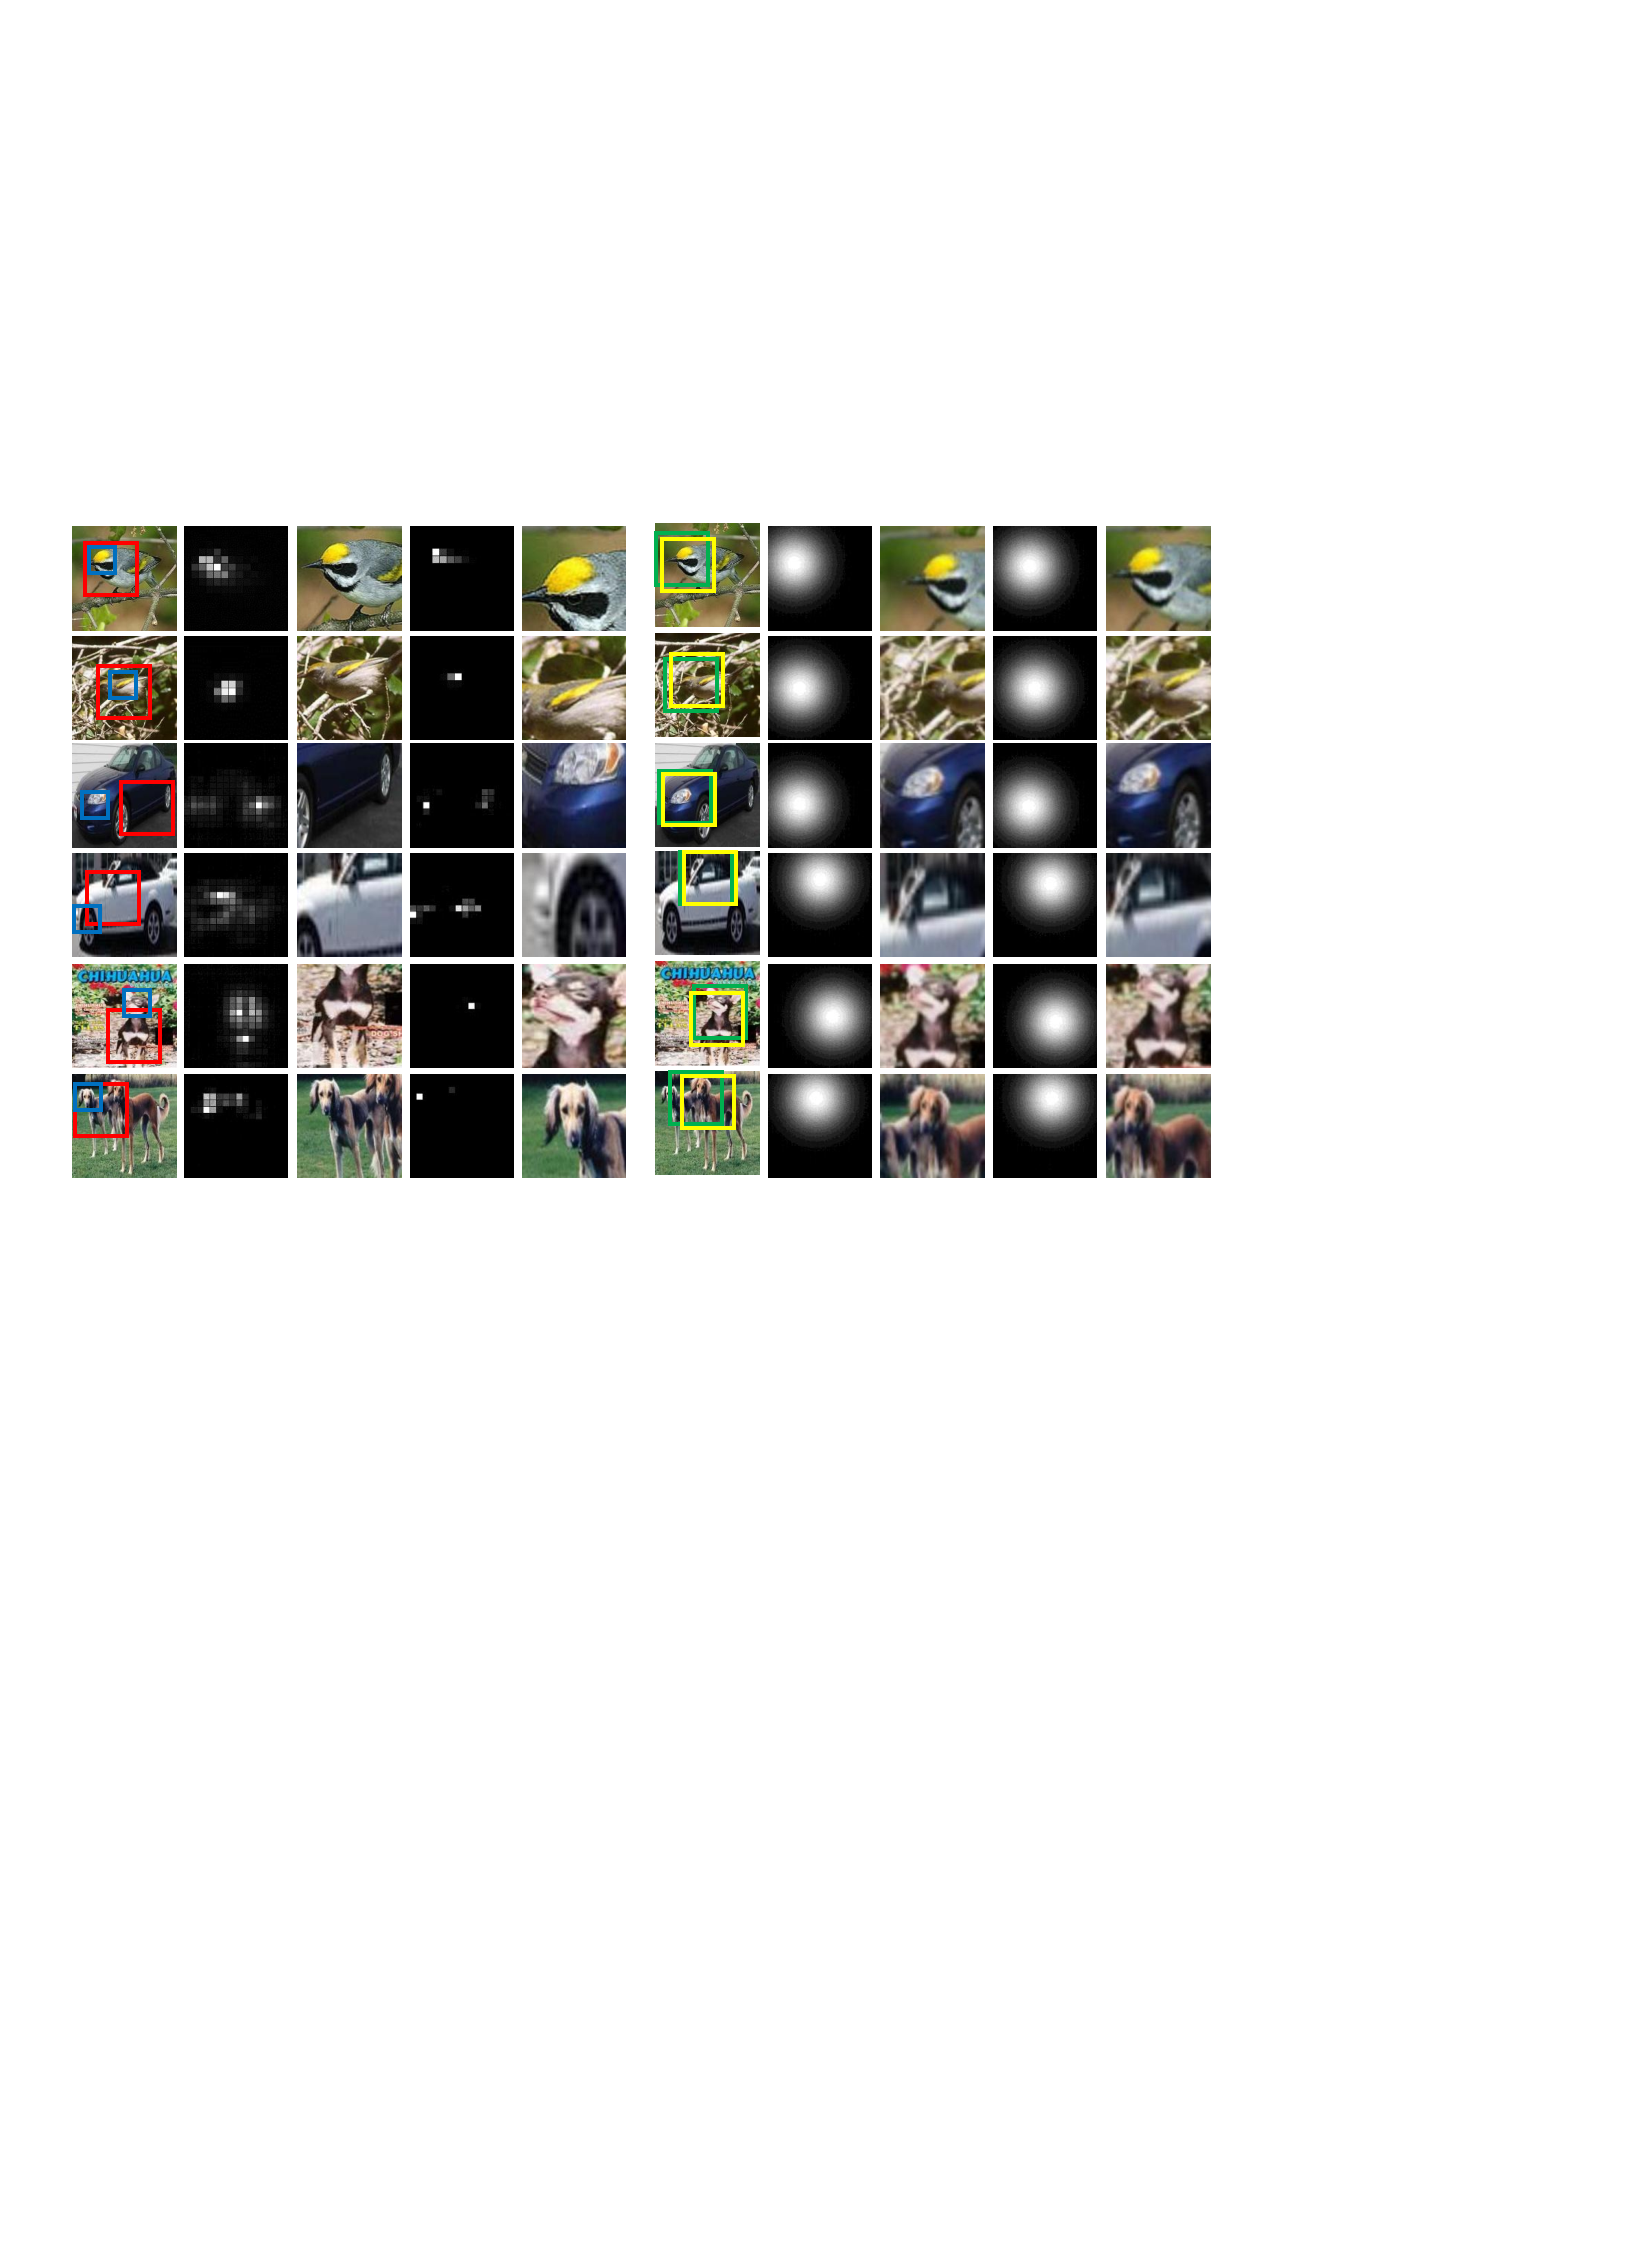
\includegraphics[scale = 0.5]{3.pdf}
\end{center}
\caption{Examples of the selected attention regions for the proposed model and  \cite{bd3}.
The first and sixth columns show the input images.
The second and the fourth columns show the attention score map outputted by the attention localization networks, which corresponds to $4\times4$ and $8\times8$ attention regions respectively (lighter color indicates higher score).
The third and the fifth columns show selected attention regions (indicated as red and blue bounding boxes in the first column).
The seventh and the ninth columns indicate the attention score maps of predicted attention regions in the two steps of recurrent attention model \cite{bd3}, respectively.
The eighth and tenth columns illustrate the corresponding selected attention regions (indicated as green and yellow bounding boxes in the six column).
}\label{fig:attention_illustration}
\vspace{-8pt}
\end{figure*}

\begin{figure*}[!t]
\begin{center}
    \subfigure[]{
    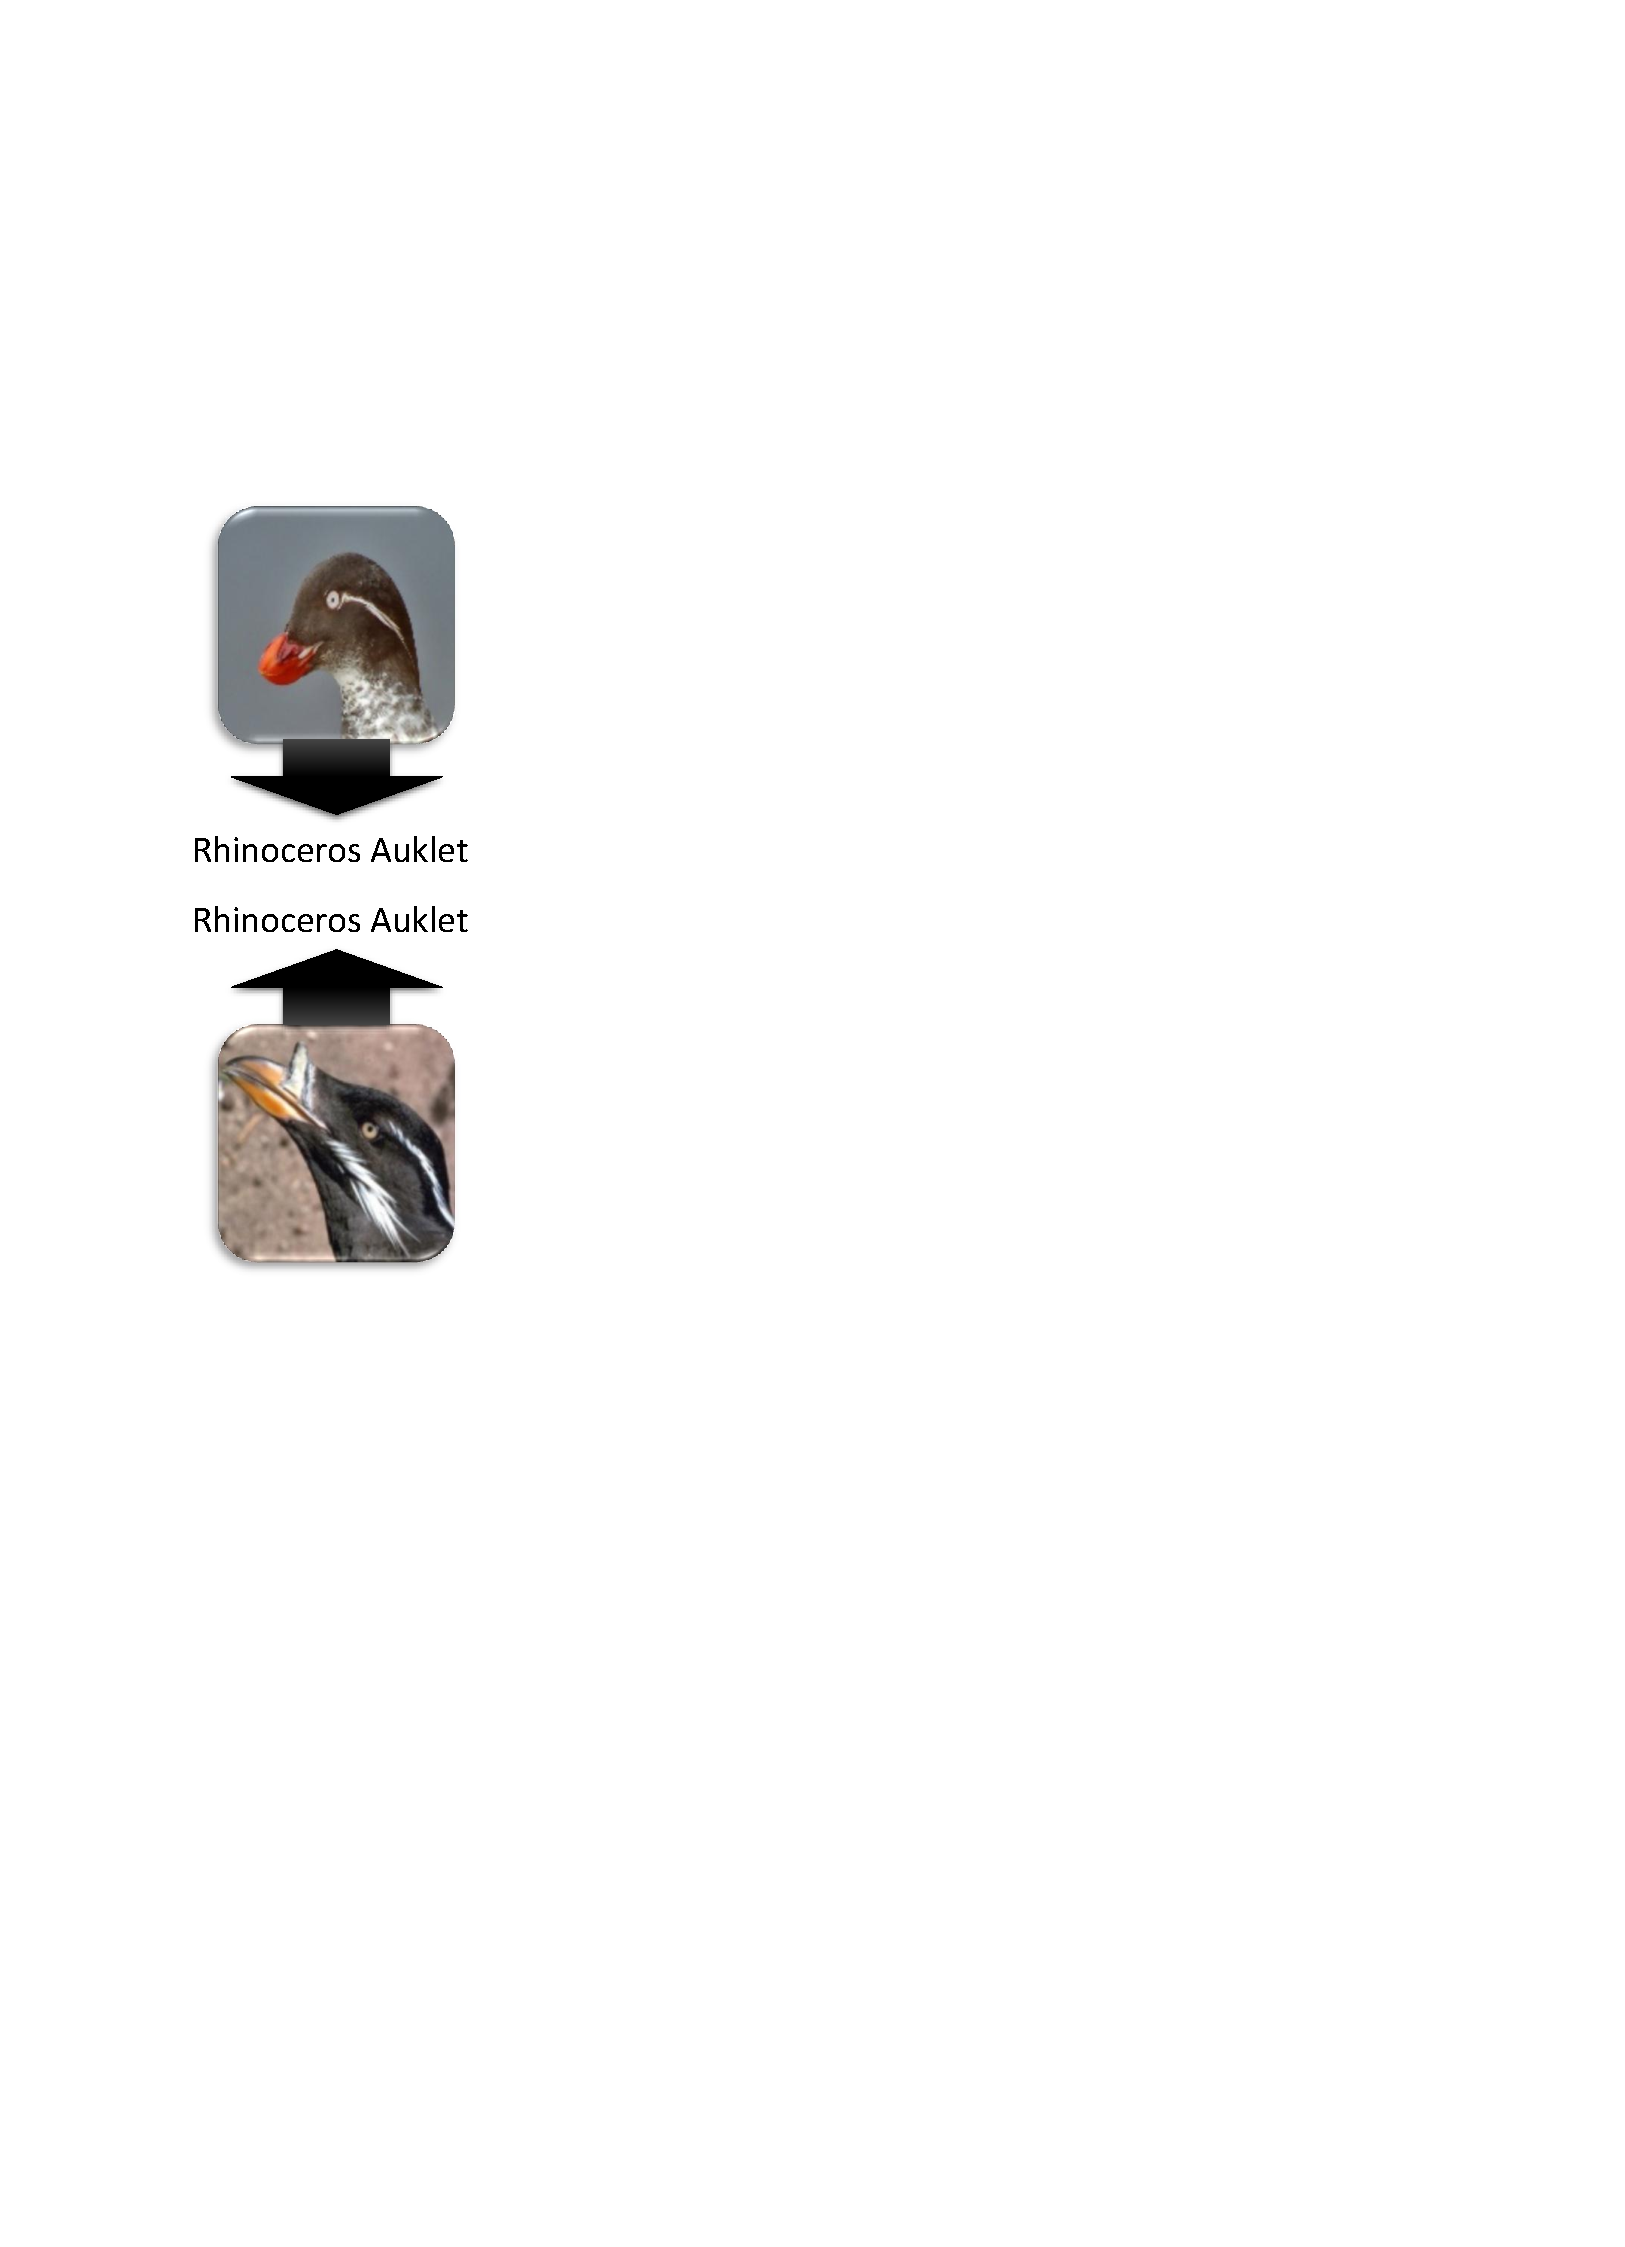
\includegraphics[scale = 0.25]{4-1.pdf}}
    \hspace{0.5in}%
    \subfigure[]{
    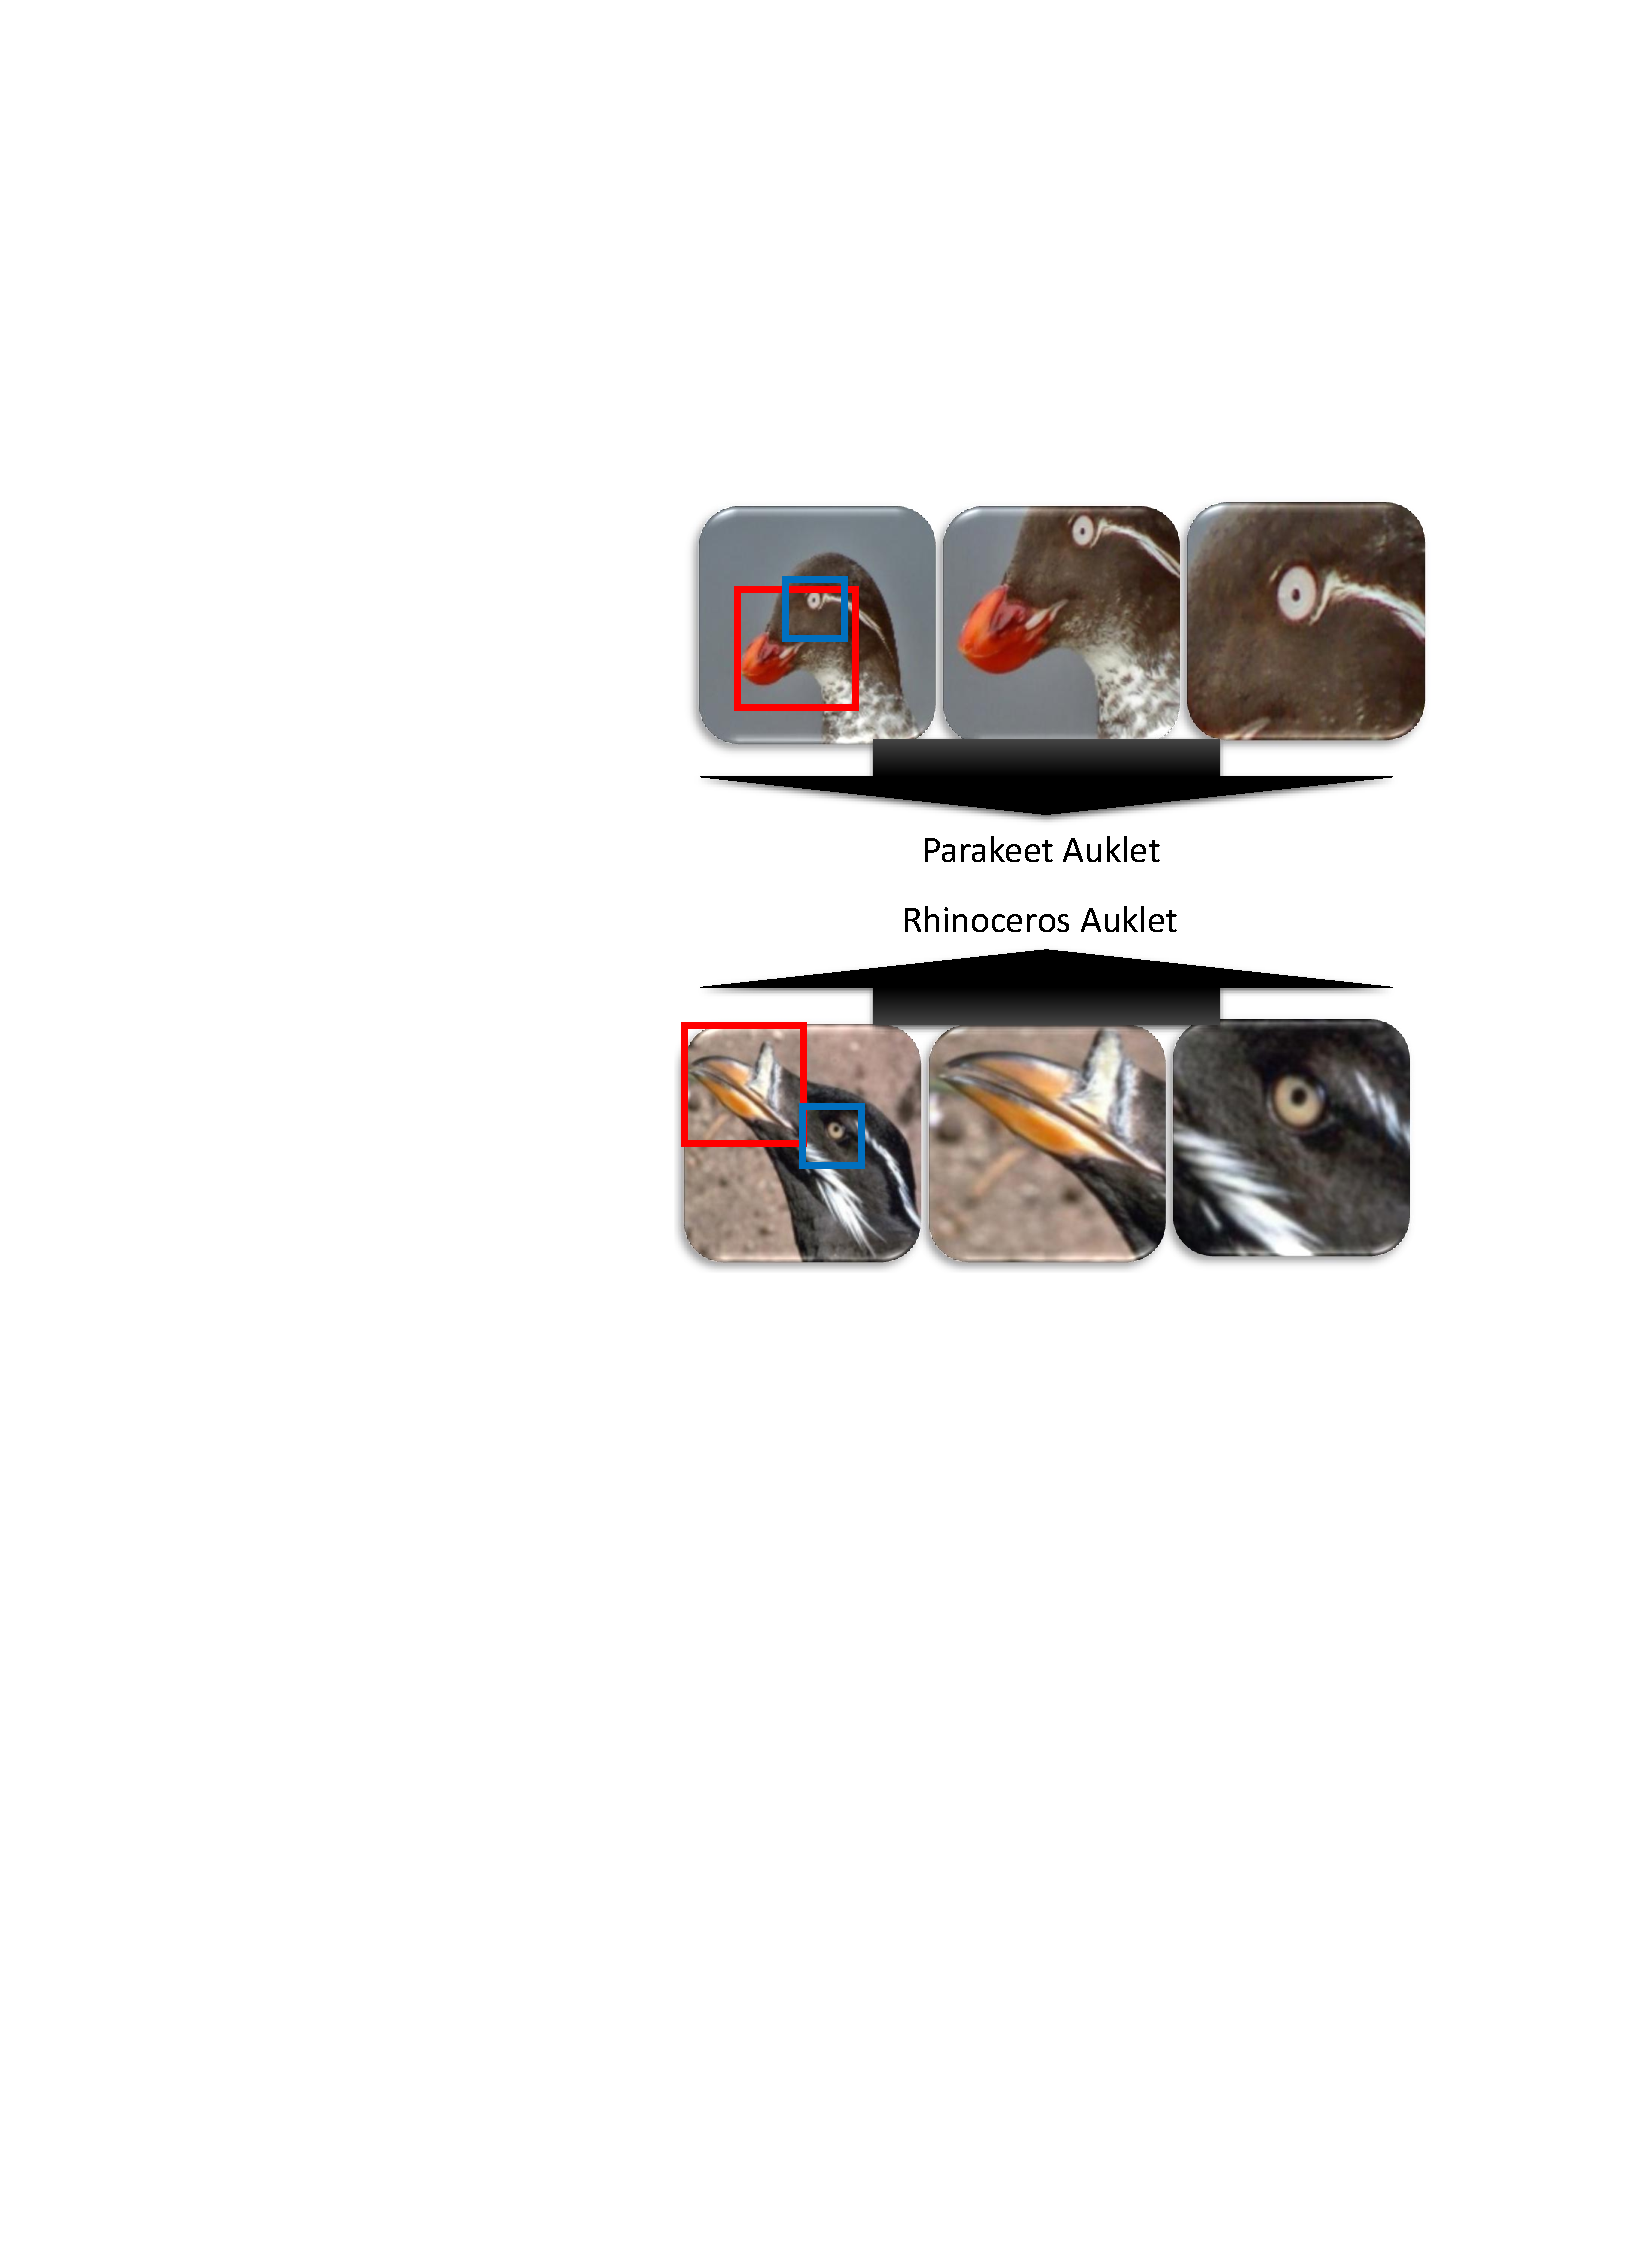
\includegraphics[scale = 0.25]{4-2.pdf}}
\end{center}
\caption{The baseline GoogLeNet misclassifies the bird in the top row of (a) as a Rhinoceros Auklet which is the category of the bird in the bottom row. The attention localization network selects the beak and eye area as attention regions, and successfully distinguishes the two birds in (b).
\vspace{-8pt}
}\label{fig:attention_illustration2}
\end{figure*}

\section{Conclusion}
In this paper, we present a novel Fully Convolutional Attention Localization Network for fine-grained recognition.
Since a fully convolutional architecture and feature sharing are utilized to improve computational efficiency,
the model is much faster than state-of-the-art reinforcement learning-based visual attention models during both training and testing.
It also achieves considerably higher recognition accuracy because it can simultaneously locate multiple object parts,
as demonstrated by the experiments on three publicly available benchmark datasets.
In the future, we will explore using differentiable attention model to further increase the training efficiency.


\bibliographystyle{splncs}
\bibliography{./IEEEabrv,./IEEEexample}
\end{document}
